
\chapter{Model Predictive Control in Single Board Heater System}
This chapter presents Model Predictive Control in Single Board Heater System done by Mr. Pratik Behera.\footnote {Copyright: Mr.Pratik Behera}
\section{Objective}
\begin{itemize}
\item To implement Model Predictive Control (MPC) in Single Board Heater System using Scilab and perform experiments using it
\item To perform experiments for various values of tuning parameters and study its effect on the system 
\end{itemize}

\section{Model Predictive Control}
An equivalent quadratic programming (QP) formulation for constrained DMC  is given as follows
\\ \\
\begin{align}
min_{U_{f}}\frac{1}{2}U_{f}(k)^{T}HU_{f}(k)+F^{T}U_{f}(k)\label{eqn1}   
  \intertext{Subject to}
  AU_{f}(k) \leq b
  \intertext{where}
\end{align}
\[
A =
\left[ {\begin{array}{cc}
 I_{qm}  \\
 -I_{qm}  \\
 \end{array} } \right]
\]
\\
\[
b =
\left[ {\begin{array}{cc}
 U^{H}  \\
 -U_{L}  \\
 \end{array} } \right]
\] \\
\begin{align}
\intertext{Also, we have outputs and manipulated variables related to state variables by}
x(k+1)=\Phi x(k) + \Gamma(k) + w(k) \\
y(k)= Cx(k) + v(k) \\
\end{align}
$\phi$ is represented by matrix A in the code, $\Gamma$ is represented as matrix B and C is represented as C matrix in the code.


\section{Working of codes}
There are three main codes, which are being used for this experiment. \emph{mpc\_init.sce} is the code which opens the xcos window, wherein, we have step block for the set-point for temperature and the fan speed. Once the values have been entered into the xcos window and the simulation is started, the \emph{scifunc} block of xcos calls the function \emph{mpc.sci} after every sampling time. The \emph{mpc.sci} in turn calls \emph{mpc\_run.sci} every time it is called by  \emph{scifunc} block. The \emph{mpc\_run.sci} code optimizes manipulated variable (heater) over control horizon and returns only the first manipulated variable (heater) value. This new heater value is then sent to the heater of the SBHS to control the temperature at the set point.
\section{Description of xcos}
When \emph{mpc\_init.sce} is executed in scilab, an xcos window opens up. The xcos window has two step input blocks. The first step input block on the left side, is for the Temperature set point and the second step input block is for the fan (disturbance variable). Also the sampling time can be entered via clock block present on the xcos. \\
For all the experiments done for this project, sampling time of 1 second was used (entered via clock block of xcos). \\
Refer to the figure below for a clear picture of the xcos.
\begin{figure}[H]
\centering
  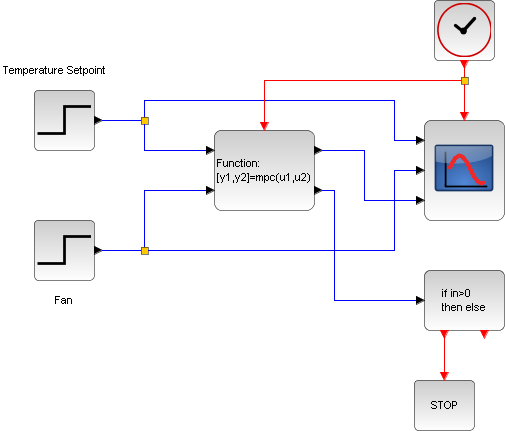
\includegraphics[width=12cm, height=10cm]{mpc/mpc_xcos.png}
  \caption{Screenshot of the xcos window with step input blocks labeled}
\end{figure}
After entering the values in the input step block, the simulation can be started. This opens up a graph, which shows the values of Temperature-set-point, fan and the actual temperature at each time instant during the simulation.


\section{Procedure to implement MPC on SBHS}
\subsection{Locally}

Change the working directory of scilab to the folder where the local mpc code are kept. Run the {\tt ser\_init.sce} file with the appropriate com port number. Then execute the file {\tt mpc\_init}. Launch xcos and execute the file {\tt mpc.xcos}. The code is listed in Section \ref{mpccodes}
\subsection{Virtually}
The step by step procedure for conducting an experiment virtually is explained in section \ref{vlabsexpt}. The required .sce file is {\tt mpc\_init.sce}.  You will find this file in the {\tt mpc} directory under {\tt virtual} folder. The necessary codes are listed in the section \ref{mpccodes}










\section{Experiments conducted to implement MPC}
Experiments were performed as shown in table above for implementation of MPC. Experiments were carried out in which both positive and negative step changes were given to the Set point and Fan (disturbance variable) and the output response was obtained by the application of MPC. Several experiments were also performed to study the effect of change in the values of q (control horizon) and tuning parameters - error and manipulated variable weighting factors. \\ \\
The details of the experiments mentioned in this report has been tabulated in the table given in the next page. The first column of the table represents the experiment version (or number). For all the outputs and their figures, we have mentioned only their experiment version (or number) to tag them. Also note that the data files for these experiments are also named as per their experiment version number. \\ \\
p and q mentioned in the table represents the prediction and control horizon respectively. \\ \\

\textbf{For graphs:} Until and unless mentioned, Graphic 1 represents the Temperature set point, Graphic 2 represents the Fan and Graphic 3 represents the Temperature. \\ \\
Also, please note that there are two types of graphs. The first graph, containing Graphic 1, Graphic 2 and Graphic 3 were directly obtained via mscope of xcos. The graph following this in all the experiments is the temperature and heater value graphs, which were obtained from the data (from the text file downloaded from the server after each experiment).
\begin{figure}[H]
\centering
  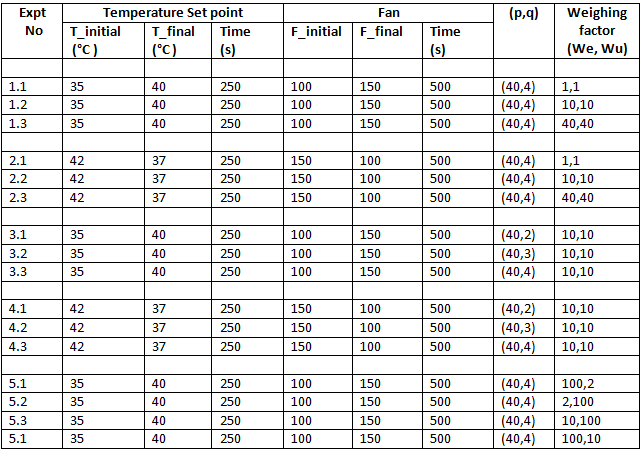
\includegraphics[width=0.7\linewidth]{mpc/table_normal.png}
  \caption{Experiments performed}
\end{figure}
All the experiments mentioned in this report has been labeled as shown in this table. This table is just a summary of all the parameters that was used for the corresponding experiment. Details on the inputs and a description of the output observed for each case has been mentioned in the corresponding section of each experiment.


\section{Positive Step Change to Set Point and Fan}
Let us consider experiment 1.1, wherein, a positive step change of 5$^\circ$ C (from 35$^\circ$ C to 40$^\circ$ C) was provided to set point at time t=250 s and a step change to fan was provided at t = 500 s, from 100 to 150. \\ \\
The graph obtained has been attached below:\\
\begin{figure}[H]
  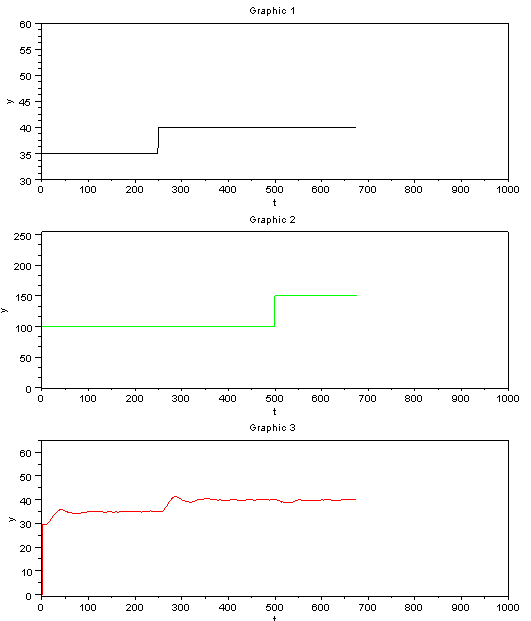
\includegraphics[width=12cm, height=15cm]{mpc/1_1.png}
  \caption{Expt 1.1}
\end{figure}
\begin{figure}[H]
  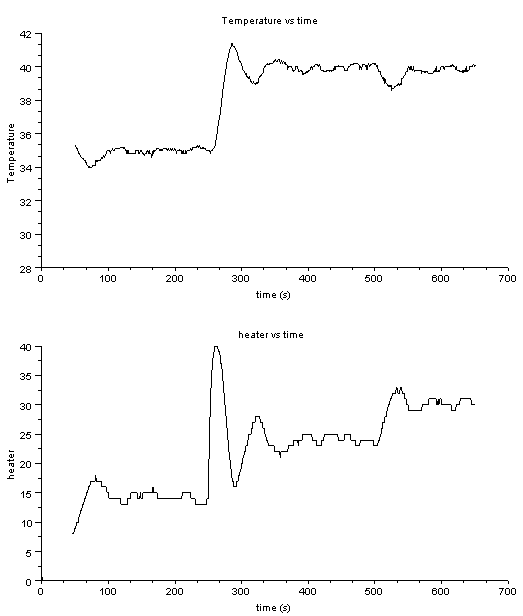
\includegraphics[width=12cm, height=15cm]{mpc/1_1_heater_final.png}
  \caption{Expt 1.1}
\end{figure}
As can, be seen above, when, the temperature set point is raised to 40 from 30, at t=250 s, the value of the heater increases, so that it can heat up the plant upto the required set point. Similarly, when the fan speed is increased at t=500s, the heater value increases yet again to maintain the same constant temperature of the SBHS blade. 


\section{Negative Step Change to Set Point and Fan}
Let us consider experiment 2.1, wherein, a negative step change of 5$^\circ$C (from 42$^\circ$C to 37$^\circ$C) was provided to set point at time t=250 s and a step change to fan was provided at t = 500 s, from 150 to 100. \\
The graph obtained has been attached below:\\
\begin{figure}[H]
  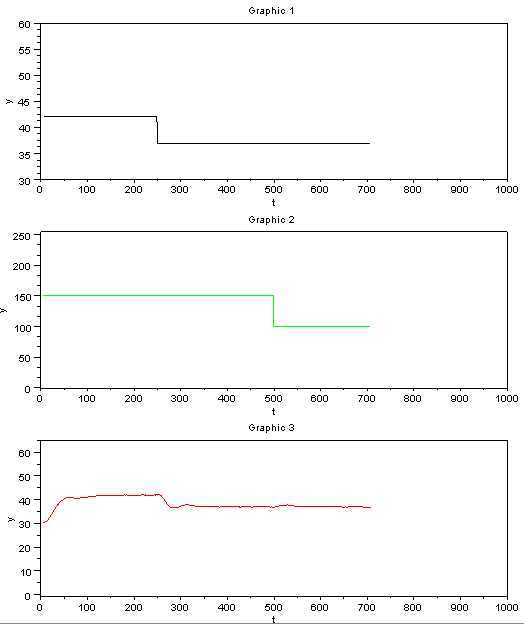
\includegraphics[width=12cm, height=15cm]{mpc/2_1.PNG}
  \caption{Expt 2.1}
\end{figure}
\begin{figure}[H]
  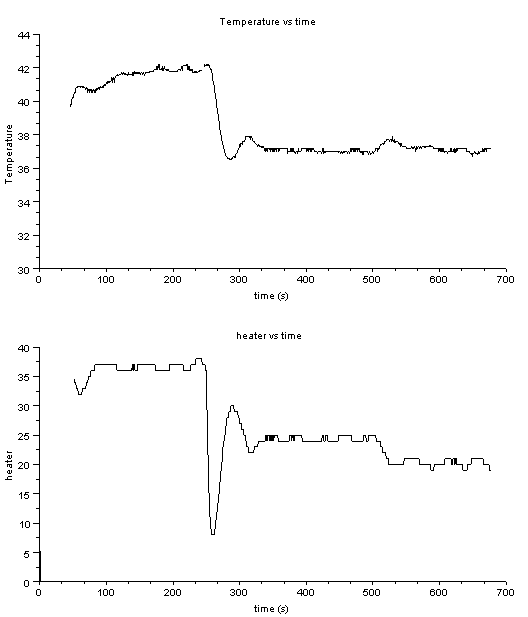
\includegraphics[width=12cm, height=15cm]{mpc/2_1_heater_final.png}
  \caption{Expt 2.1}
\end{figure}
As can be seen from the graphs above, when the temperature set point drops at t=250 s, the value of the heater too falls, so that the plant (SBHS blade) can cool down to the required set point. Similarly, when the fan speed was decreased at t=500s, the heater value decreased yet again to maintain the same constant temperature of the SBHS blade.


\section{Effect of Tuning parameters: Weighting factors, We and Wu}
We also, conducted several experiments in order the study the effect of the value of Weighting factors (both error,We and manipulated variable,Wu). We used weighting factors to be 1, 10 and 40 for both positive and negative step changes to both set point and fan (as has been summarized in Table 1). Also, experiments were done for different values of We and Wu. The results have been shown in the following graph. \\
\section{For same factor of We and Wu}
\subsection{Positive Step Change and (We, Wu)=(1,1) (Expt 1.1)}
\begin{figure}[H]
  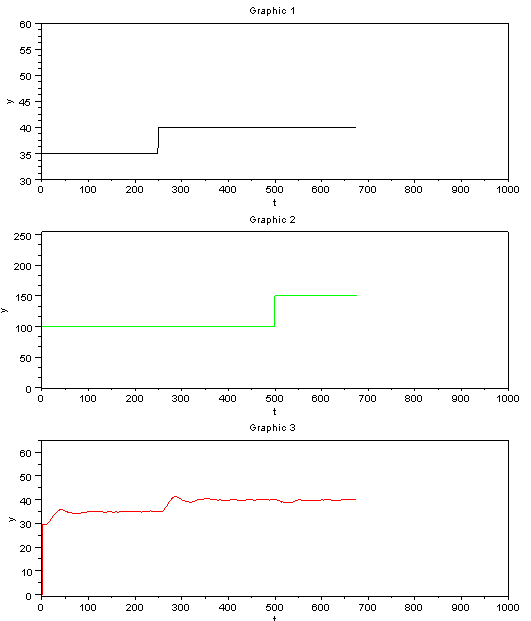
\includegraphics[width=12cm, height=15cm]{mpc/1_1.png}
  \caption{Expt 1.1}
\end{figure}
Here we can clearly see the expected output. Providing a positive step to temperature set point at 250 seconds, increased heater value as per the control effort put in by MPC. A positive step in fan at 500 seconds, decreased the temperature below its set point and hence heater value increased to take the temperature close to its setpoint. \\
This will be clear from the heater graph attached next.
\begin{figure}[H]
  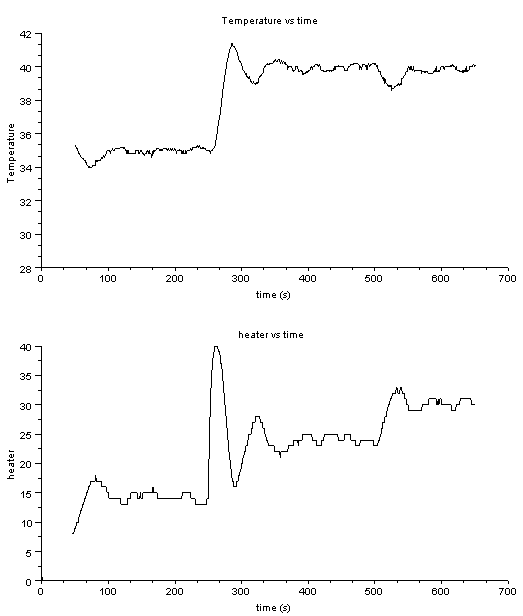
\includegraphics[width=12cm, height=15cm]{mpc/1_1_heater_final.png}
  \caption{Expt 1.1}
\end{figure}
As can be clearly seen, the heater graph follows the expected trend that we talked of in the last page. Also, note that the temperature variation can be clearly seen from this graph. \\
This graph shows the result for the case, where we had same weighting factors for both error and manipulated variables (We and Wu). We will now see if changing both of these is going to have any effect on the control behavior. \\
So, we now try an experiment with both We and Wu increased to 10.


\subsection{Positive Step Change and (We, Wu)=(10,10) (Expt 1.2)}
\begin{figure}[H]
  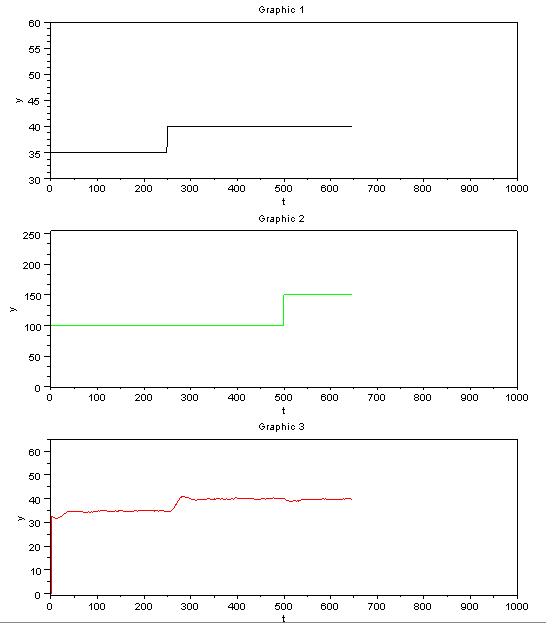
\includegraphics[width=12cm, height=15cm]{mpc/1_2.png}
  \caption{Expt 1.2}
\end{figure}
Using the same logic as has been explained in the last section, we expected to see similar temperature and heater value profiles for the positive step change in temperature set point and the fan. (Heater graph is shown in the next page along with the temperature on an expanded scale). \\
In this experiment, we increased We and Wu both to 10 from 1 and wish to observe if this changes the response of the plant.
\begin{figure}[H]
  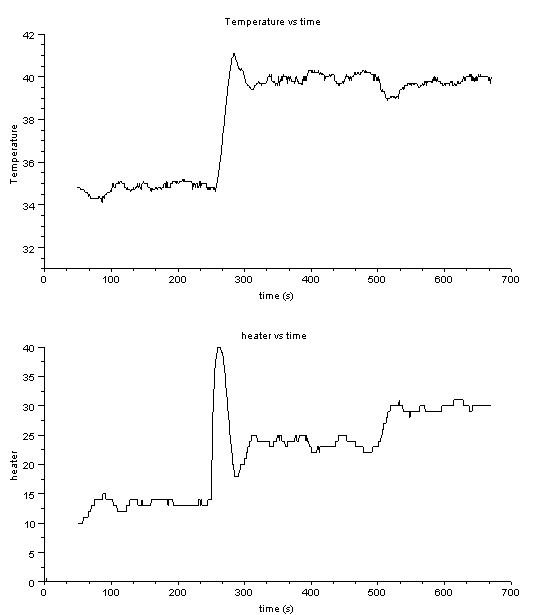
\includegraphics[width=12cm, height=15cm]{mpc/1_2_heater_final.png}
  \caption{ Expt 1.2}
\end{figure}
The results here are almost the same as that mentioned in the last section (where We and Wu both were 1). So, we can for the time being keep in mind that We and Wu isn't actually much affected the output. We now will carry out the experiment for even higher We and Wu (say 40) and see if it really does affect the output much.


\subsection{Positive Step Change and (We, Wu)=(40,40) (Expt 1.3)}
\begin{figure}[H]
  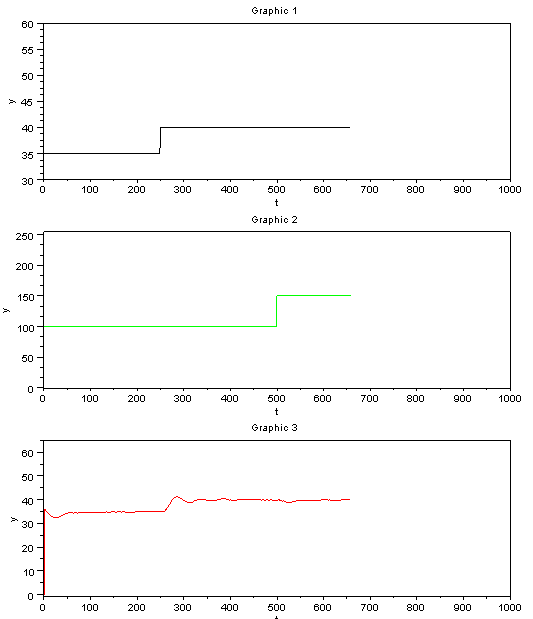
\includegraphics[width=12cm, height=15cm]{mpc/1_3.PNG}
  \caption{ Expt 1.3}
\end{figure}
\begin{figure}[H]
  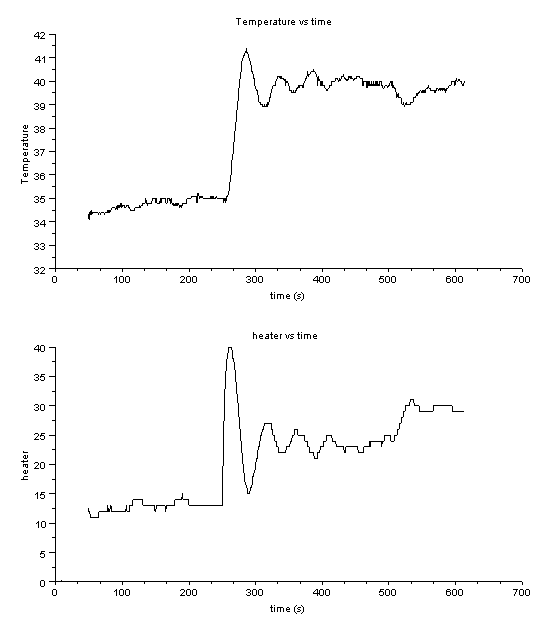
\includegraphics[width=12cm, height=15cm]{mpc/1_3_heater_final.png}
  \caption{Expt 1.3}
\end{figure}
Even the results with We and Wu as 40 doesn't show much difference. They are more or less similar looking as the last two experiment's results.


\subsection{Negative Step Change and (We,Wu)=(1,1) (Expt 2.1) }
\begin{figure}[H]
  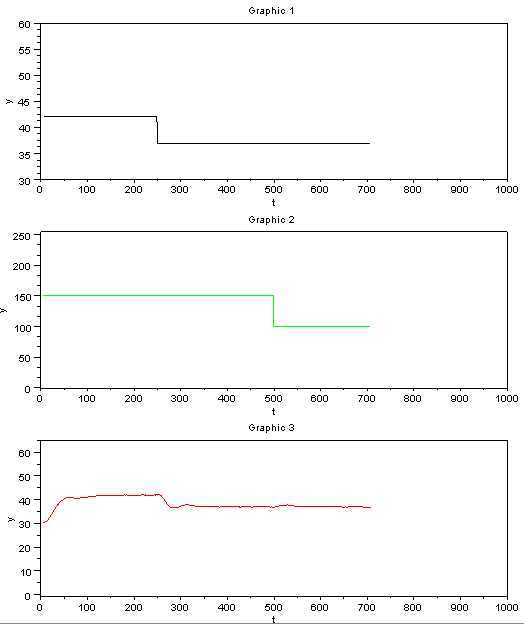
\includegraphics[width=12cm, height=15cm]{mpc/2_1.PNG}
  \caption{Expt 2.1}
\end{figure}
Here we expect somewhat similar results as was the case with positive step in temperature set point.
\begin{figure}[H]
  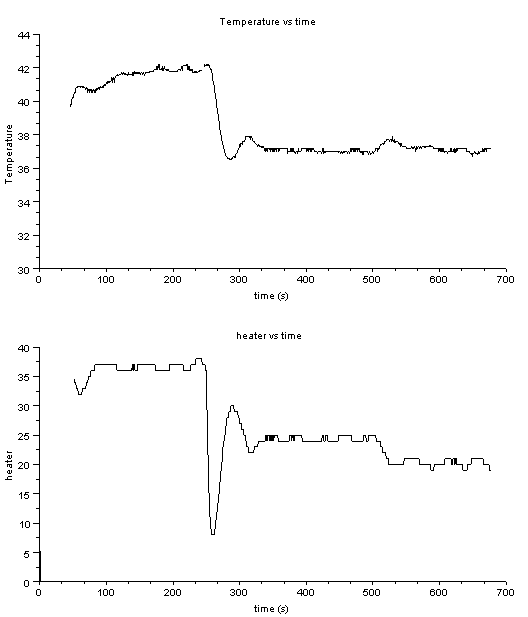
\includegraphics[width=12cm, height=15cm]{mpc/2_1_heater_final.png}
  \caption{ Expt 2.1}
\end{figure}
We can very clearly make out that the results follow the trends as was explained for the negative step input in the section 5.2


\subsection{Negative Step Change and (We, Wu)=(10,10) (Expt 2.2) }
\begin{figure}[H]
  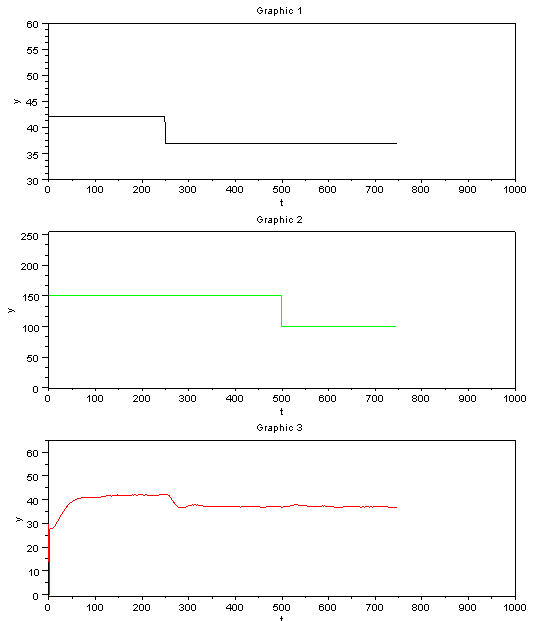
\includegraphics[width=12cm, height=15cm]{mpc/2_2.PNG}
  \caption{Expt 2.2}
\end{figure}
\begin{figure}[H]
  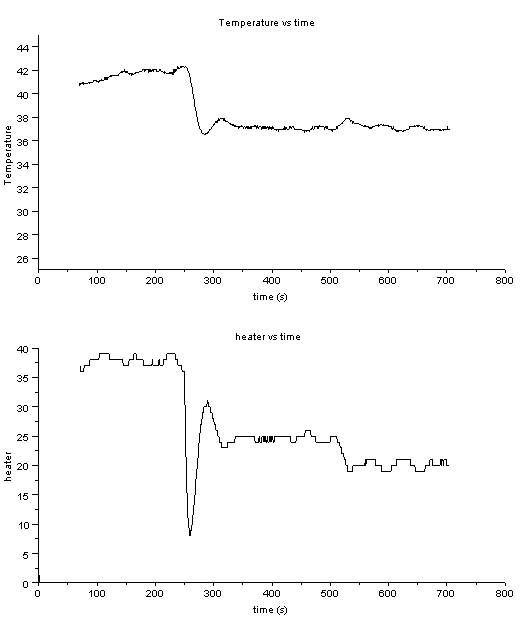
\includegraphics[width=12cm, height=15cm]{mpc/2_2_heater_final.png}
  \caption{Expt 2.2}
\end{figure}


\subsection{Negative Step Change and (We, Wu)=(40,40) (Expt 2.3)}
\begin{figure}[H]
 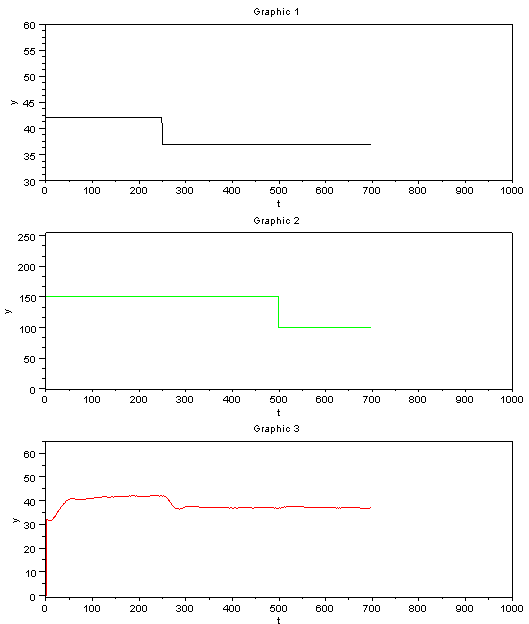
\includegraphics[width=12cm, height=15cm]{mpc/2_3.PNG}
  \caption{Expt 2.3}
\end{figure}
\begin{figure}[H]
  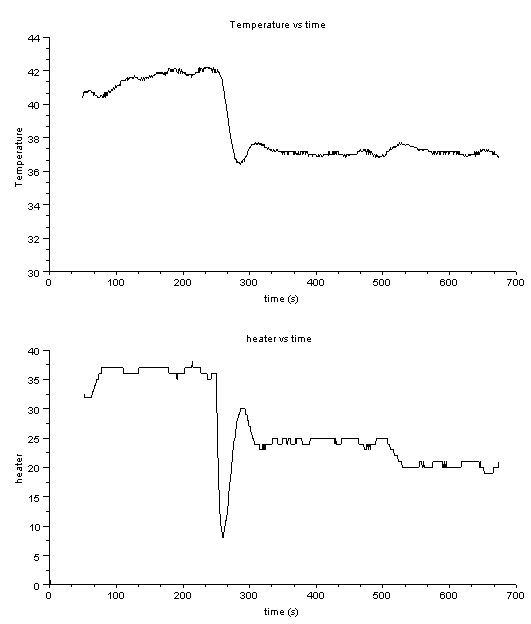
\includegraphics[width=12cm, height=15cm]{mpc/2_3_heater_final.png}
  \caption{ Expt 2.3}
\end{figure}


\section{For different We and Wu factors}
We very clearly see that using the same values of We and Wu is not making much difference in the control response. So, will now be trying different values for We and Wu.
\subsection{We =100 and Wu = 2 (Expt 5.1) }
\begin{figure}[H]
  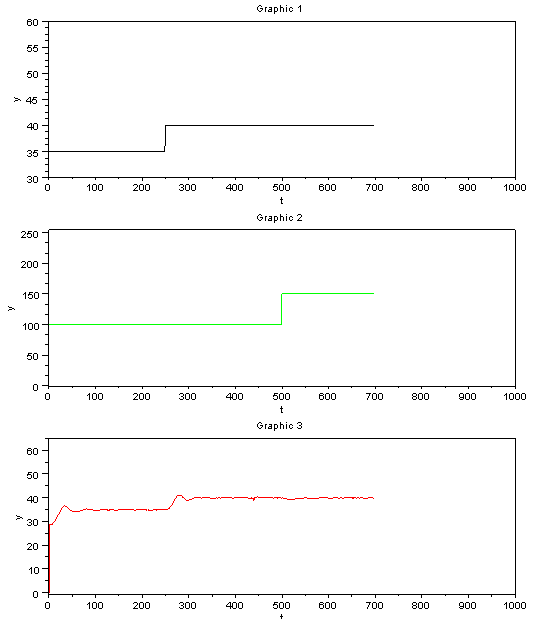
\includegraphics[width=12cm, height=15cm]{mpc/5_1.PNG}
  \caption{Expt 5.1}
\end{figure}
Here, we have used We as 100 and Wu as 2. The response after the positive step in temperature set point is slightly oscillatory. The temperature very well stabilzes at the required setpoint. The settling time observed is fairly low.
\begin{figure}[H]
  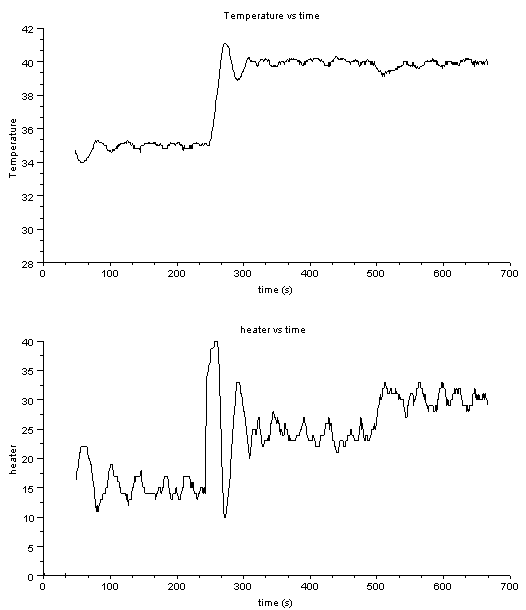
\includegraphics[width=12cm, height=15cm]{mpc/5_1_heater_final.png}
  \caption{Expt 5.1}
\end{figure}
Now having seen the results of this experiment, we would like to check the possible effect of reversing the values of We and Wu. So, we conduct the next experiment, in which we have We as 2 and Wu as 100.


\subsection{We =2 and Wu = 100 (Expt 5.2) }
\begin{figure}[H]
  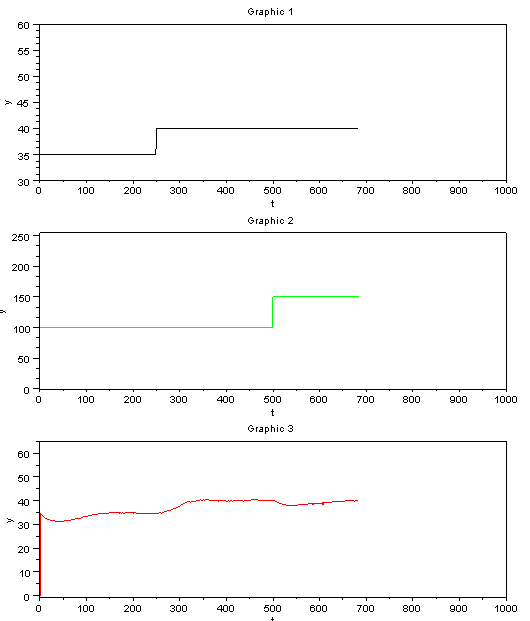
\includegraphics[width=12cm, height=15cm]{mpc/5_2.PNG}
  \caption{Expt 5.2}
\end{figure}
With increase in Wu, we observe that the temperature stabilzes at the required stepoint, but the settling time for reaching that setpoint increases. Also, the response is not oscillatory. This result can be very clearly seen in the following temperature and heater graph.
\begin{figure}[H]
  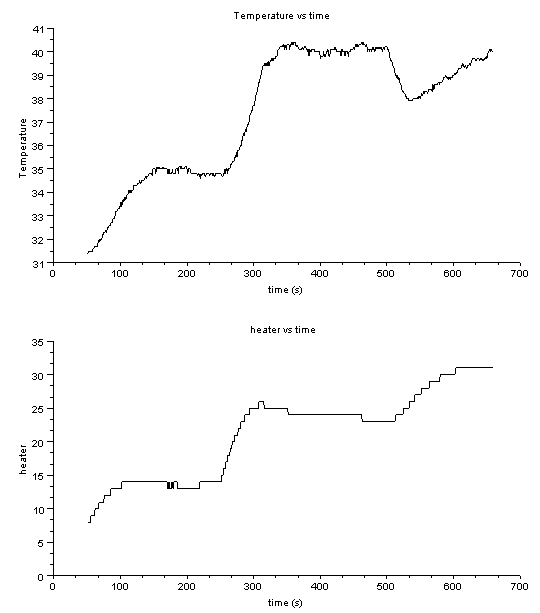
\includegraphics[]{mpc/5_2_heater_final.png}
  \caption{Expt 5.2}
\end{figure}


\subsection{We =10 and Wu = 100 (Expt 5.3)}
Having seen the effect of low We and high Wu (in the last section), we would like to see what happens if We is slightly increased keeping Wu the same. For this we increase the value of We to 10 and keep Wu at constant 100.
\begin{figure}[H]
  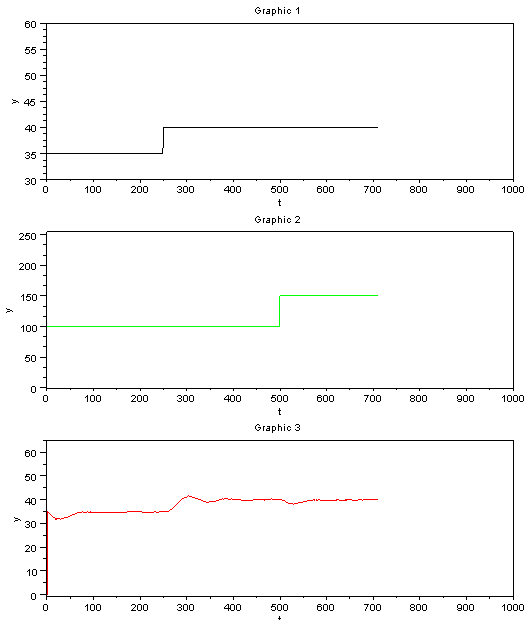
\includegraphics[width=12cm, height=15cm]{mpc/5_3.PNG}
  \caption{Expt 5.3}
\end{figure}
We observe that this experiments performs better than in the last section (where We was 2). It is slighly oscillatory and also, the settling time decreased much as compared to last experiment.
\begin{figure}[H]
  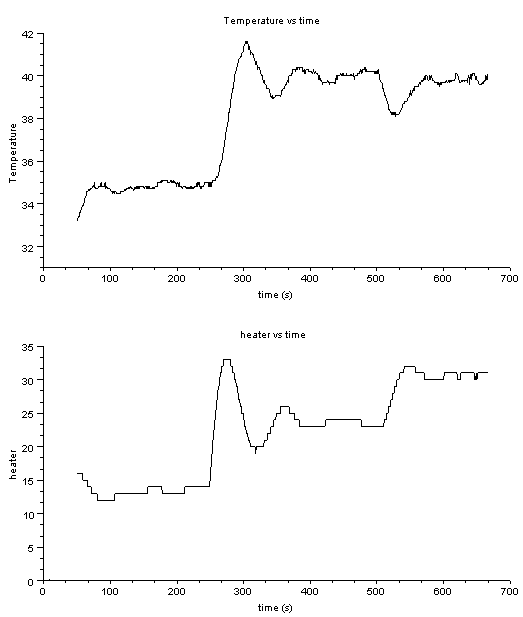
\includegraphics[width=12cm, height=15cm]{mpc/5_3_heater_final.png}
  \caption{Expt 5.3}
\end{figure}


\subsection{We =100 and Wu = 10 (Expt 5.4)}
We now do a similar study for the case of Wu. We increase the value of Wu to 10, keeping We constant at 100.
\begin{figure}[H]
  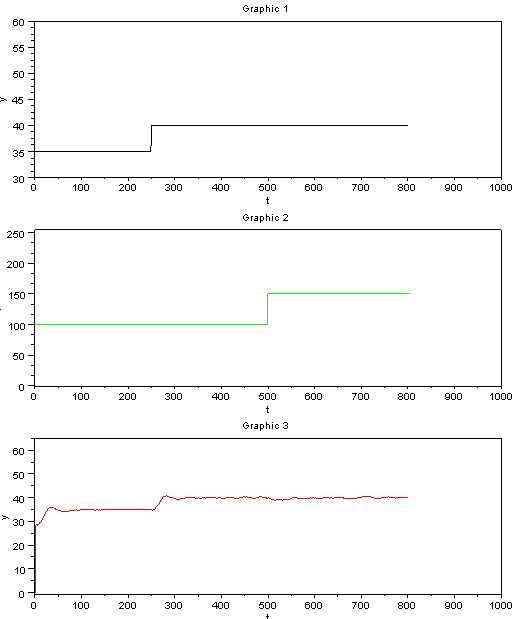
\includegraphics[width=12cm, height=15cm]{mpc/5_4.PNG}
  \caption{Expt 5.4}
\end{figure}
As is clear from the figure, we see slightly lesser oscillations compared to the case when We was 100 and Wu was 2. Settling time more or less remained the same.
\begin{figure}[H]
  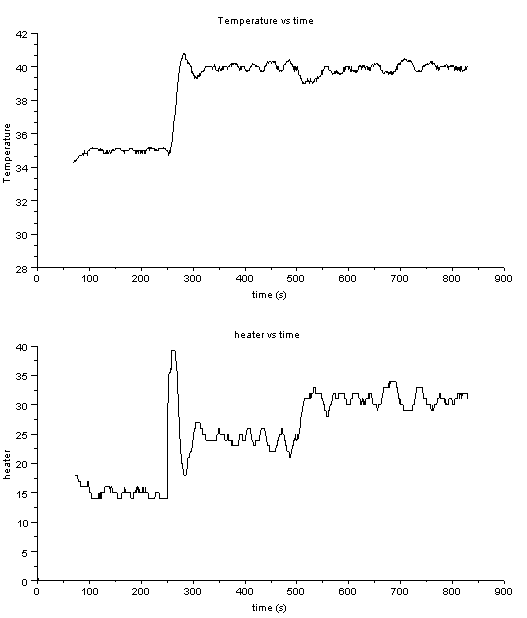
\includegraphics{mpc/5_4_heater_final.png}
  \caption{Expt 5.4}
\end{figure}


\section{Conclusion on Weighting factor experiments}
\textbf{For experiments with same values of We and Wu}:
\begin{itemize}
\item Not much difference was seen in heater value trends and temperature value trends for all the experiments performed above.
\item Reason for this will be clear from the discussion on the trends mentioned below (for experiments with different values of We and Wu)
\end{itemize}
\textbf{For experiments with different values of We and Wu}:
\begin{itemize}
\item Keeping We as large (around 100) and Wu as small (2) shows better performance as compared to the case when the values are kept the other way around.
\item With We very small (say around 1-2), oscillations are less, and the settling time observed was found to be more.
\item With increase in We, the oscillations were observed to increase and the settling time was found to reduce and hence, better control was observed.
\item So, with increase in We, any error is quickly dealt with, because with increase in We, we are actually increasing the significance of change of temperature in deciding the control action.
\item With increase in Wu, oscillations reduced and the settling time was found to increase and hence, less preferred.
\end{itemize}
So, the best performance is obtained for the cases with high We and low Wu.


\section{Effect of Control Horizon Paramter, q}
We also tried to study the effect of change of control horizon (q) on the response of the SBHS to step change in Setpoint and disturbance variable. Generally the value of q (control parameter) is taken somewhere between 2 to 5. So, we performed our SBHS experiment for values of q as 2, 3 and 4 (as suggested by Mr Prashant Gupta). \\ \\
Both positive and negative step change experiments for temperature set point and disturbance variable (fan) was performed for the sake of completeness. The results obtained thereby has been mentioned in form of graphs in this section. The overall conclusion over these experiments has been mentioned in the conclusion of this part.

\section{For positive step change in Set point and Fan speed }
\subsection{For q =2 (Expt 3.1) }
\begin{figure}[H]
  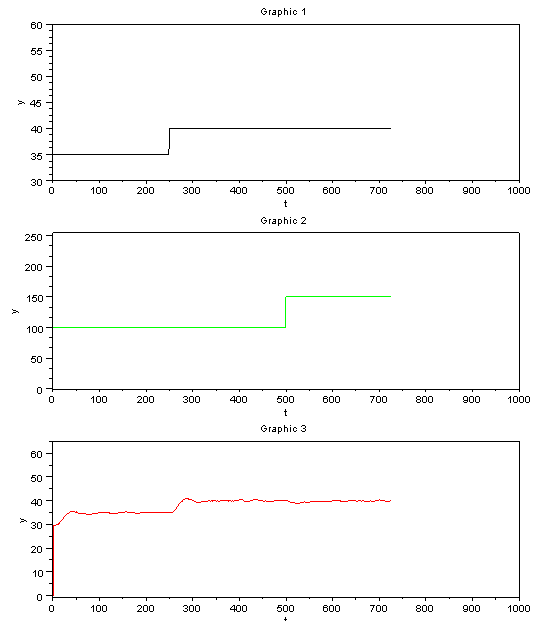
\includegraphics[width=12cm, height=15cm]{mpc/3_1.PNG}
  \caption{Expt 3.1}
\end{figure}
\begin{figure}[H]
  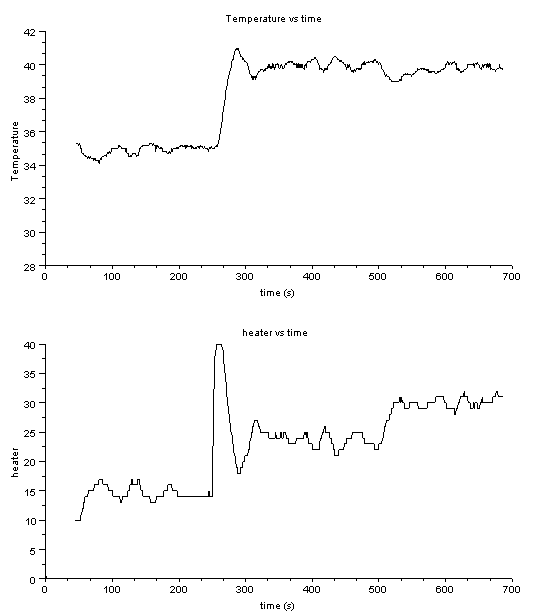
\includegraphics[width=12cm, height=15cm]{mpc/3_1_heater_final.png}
  \caption{Expt 3.1}
\end{figure}


\subsection{For q =3 (Expt 3.2) }
\begin{figure}[H]
  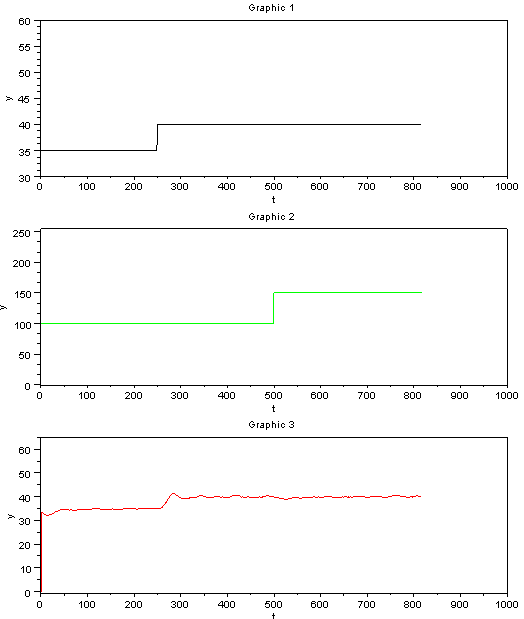
\includegraphics[width=12cm, height=15cm]{mpc/3_2.PNG}
  \caption{Expt 3.2}
\end{figure}
\begin{figure}[H]
  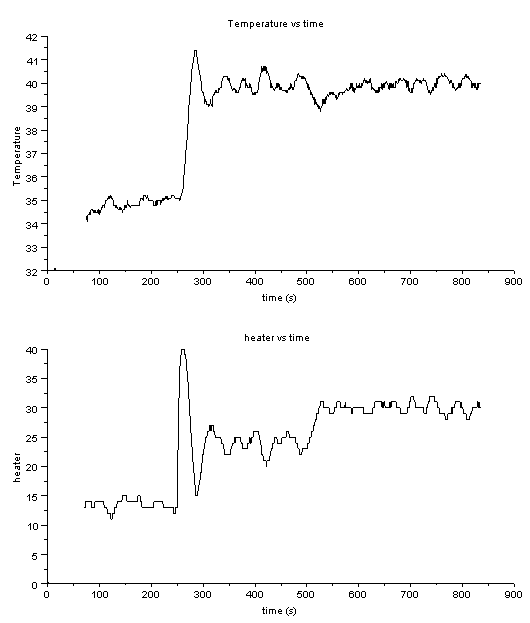
\includegraphics[width=12cm, height=15cm]{mpc/3_2_heater_final.png}
  \caption{Expt 3.2}
\end{figure}


\subsection{For q =4 (Expt 3.3) }
\begin{figure}[H]
  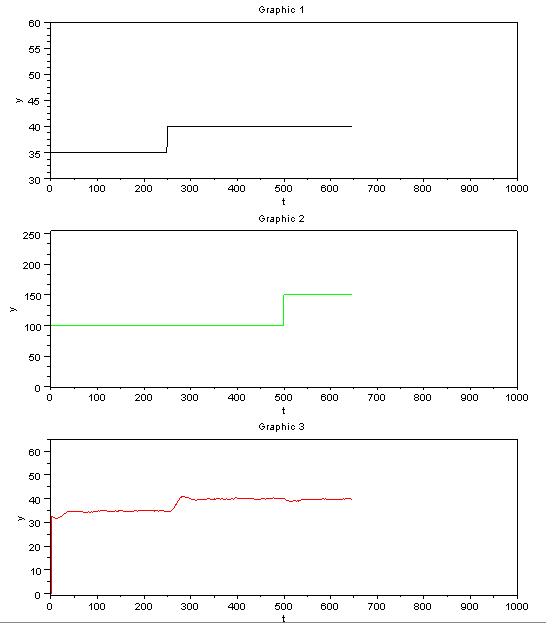
\includegraphics[width=12cm, height=15cm]{mpc/3_3.PNG}
  \caption{Expt 3.3}
\end{figure}
\begin{figure}[H]
  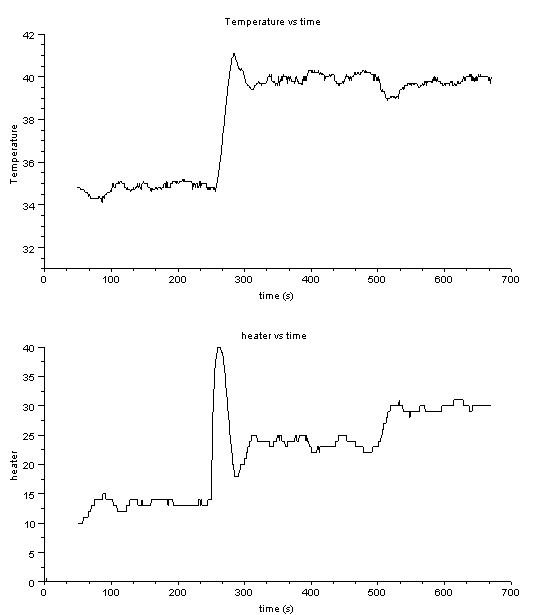
\includegraphics[width=12cm, height=15cm]{mpc/3_3_heater_final.png}
  \caption{Expt 3.3}
\end{figure}


\section{For negative step change in Set point and Fan speed }
\subsection{For q =2 (Expt 4.1) }
\begin{figure}[H]
  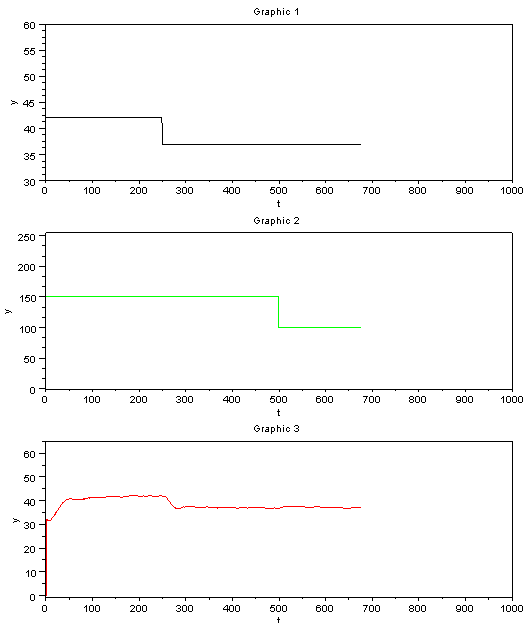
\includegraphics[width=12cm, height=15cm]{mpc/4_1.PNG}
  \caption{Expt 4.1}
\end{figure}
\begin{figure}[H]
  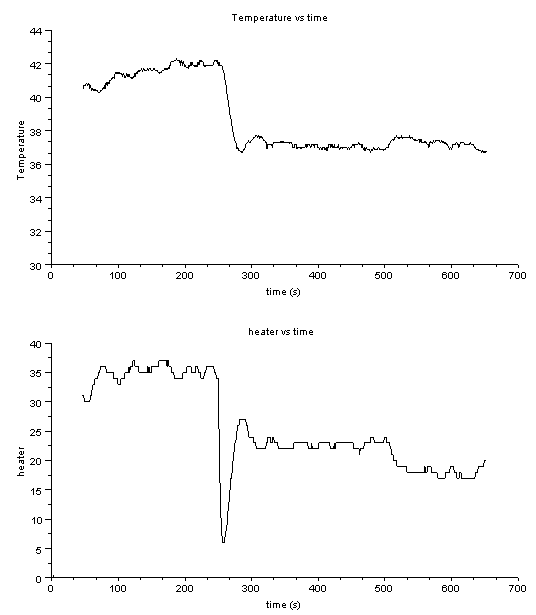
\includegraphics[width=12cm, height=15cm]{mpc/4_1_heater_final.png}
  \caption{Expt 4.1}
\end{figure}


\subsection{For q =3 (Expt 4.2) }
\begin{figure}[H]
  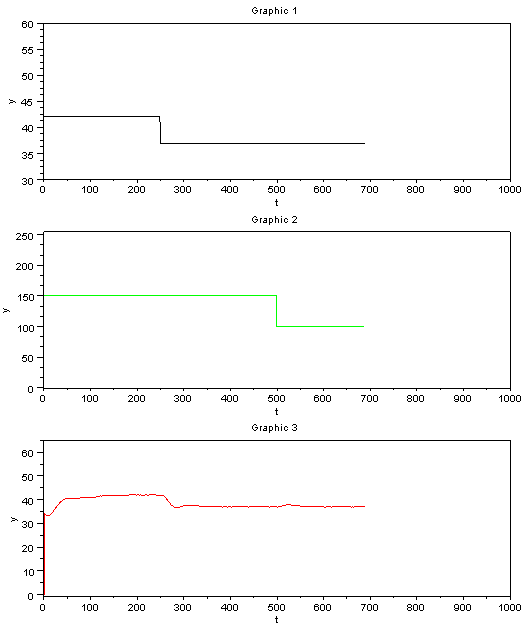
\includegraphics[width=12cm, height=15cm]{mpc/4_2.PNG}
  \caption{Expt 4.2}
\end{figure}
\begin{figure}[H]
  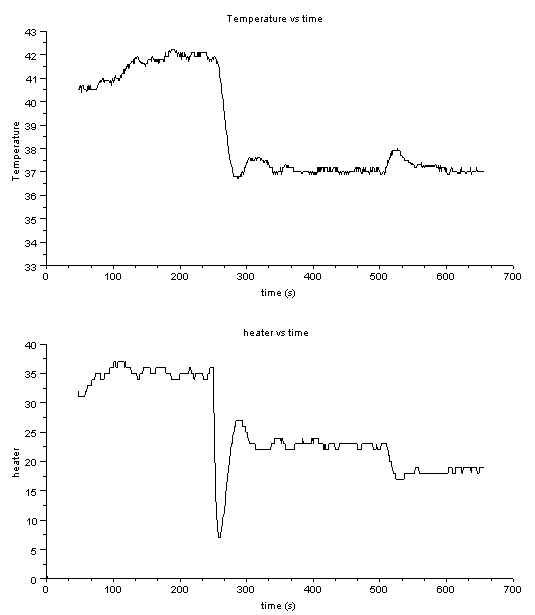
\includegraphics[width=12cm, height=15cm]{mpc/4_2_heater_final.png}
  \caption{Expt 4.2}
\end{figure}


\subsection{For q =4 (Expt 4.3) }
\begin{figure}[H]
  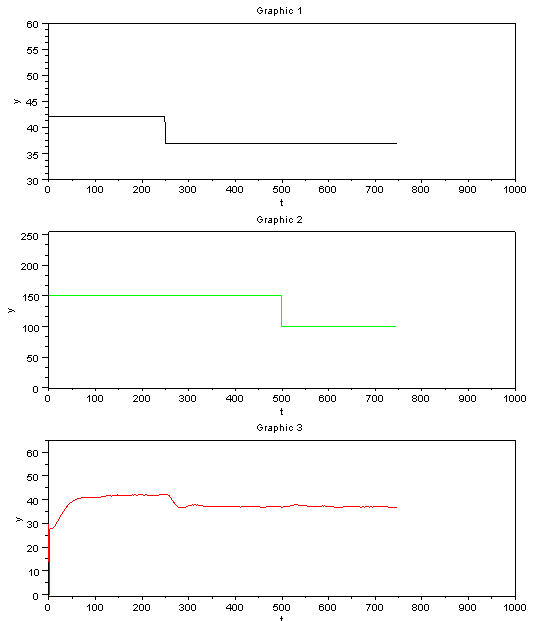
\includegraphics[width=12cm, height=15cm]{mpc/4_3.PNG}
  \caption{Expt 4.3}
\end{figure}
\begin{figure}[H]
  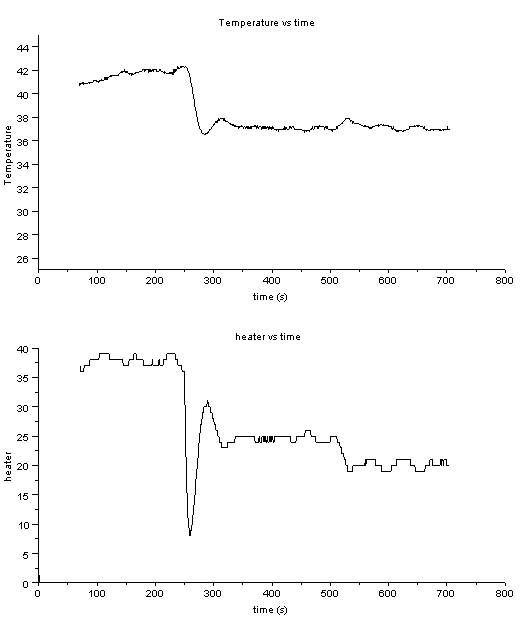
\includegraphics[width=12cm, height=15cm]{mpc/4_3_heater_final.png}
  \caption{Expt 4.3}
\end{figure}


\section{Conclusion on the effect of Control Horizon parameter }
\begin{itemize}
\item The effect of change in q isn’t very distinct in the experiments performed.
\item While we are calculating the optimized value of manipulated variable at a time, the number of manipulated input moves is increasing as we are increasing the q value. 
\item But, only the first value of the optimized manipulated variable vector is used for control. 
\item Increase in q is only increasing the length of the manipulated variable vector which is to be optimized.
\item Since, only the first value of manipulated variable vector is used, which itself lies in some specified range, the effect of changing q isn’t very significant for SBHS.
\item Also, SBHS system is a simple system with very few variables (as compared to real life industrial systems).
\item Ideally, the value of q is to be maintained at 3 or 4.
\end{itemize}



\section{Conclusion for MPC project}
The objective of this project, ie, implementing Model Predictive Control in Single Board Heater System using Scilab was successfully achieved. Several experiments were successfully performed using the developed SCILAB MPC algorithm for both positive and negative step changes in both temperature-set-point and the disturbance variable (fan). 
\\ \\ 
In addition to the above objective, we also tried studying the effect of weighting factors (tuning parameter) and control horizon parameter. We observed and concluded that increase in values of We (error weighting factor), increases oscillations and decreases settling time, while decrease in We leads to opposite effect. Wu (manipulated variable weighting factor), on the other hand has an opposite effect. It decreases oscillations and increases settling time with increase in its value. Hence, better control is obtained for high value of We and low value of Wu.
\\ \\
Thus, with this project, we were able to implement MPC successfully and also were able to comment on the general preferred tuning parameters (weighting factors for error and manipulated variable).
\\ \\

\section{Acknowledgement }
Firstly, I would like to thank Prof Moudgalya Kannan, for giving me this opportunity to undertake MPC project on SBHS. This project, which involved implementing Model Predictive Control in SBHS using SCILAB, was very interesting and provided an excellent learning opportunity. For developing the MPC algorithm, lecture notes on Model Predictive Control by Prof Sachin Patwardhan too were extremely helpful. Also, I got to learn a lot from the speaking tutorials of SCILAB and LaTeX, which had to be referred to for the completion of this project. Over and above this, it was very encouraging to see the experiments working perfectly with the developed Model Predictive Control algorithm.
\\ \\
I would also like to sincerely thank Mr Prashant Gupta, without whom, this project would not have been splendidly completed. I would like to thank him for the time he spent explaining the concepts, clearing the doubts and suggestions for the experiments to implement MPC.
\\ \\

\section{Appendix}
\section{Appendix 1: General Information on Experiments for this Project}
All the experiments for this project was performed remotely on SBHS 12, using a sampling time of 1 second. Basic codes (mpc\_init.sce and mpc.sci) was taken from moodle for this course. Code for implementing MPC was written in scilab and has been mentioned in the report. \\ \\
Scilab Version used: 5.2.2 \\
SBHS number: 12 (remotely used) \\
Sampling time: 1 second \\ \\
\emph{For graphs}: Until and unless mentioned, Graphic 1 represents the Temperature set point, Graphic 2 represents the Fan and Graphic 3 represents the Temperature.

\section{Appendix 2: Values of State Space matrices}
Initially, open loop experiment was performed, and Plant Transfer function was obtained. For the open loop experiment, a step change in heater from 15 to 25 units at t =200 seconds was provided (sampling time 1s). The response data was fitted to a first order transfer function with a time delay and the following was observed: \\
Kp=0.37, time constant = 45s and delay = 7s. \\ \\

Using the above, we obtained the plant transfer function: 
\begin{align}
G_{p}=\frac{0.37}{1+45s}e^{-7s} \label{eqn2}
\end{align}
\\
\textbf{Scilab Method to calculate State Space matrices}\\
State space matrices for a transfer function can be calculated as follows using Scilab: \\
\lstinputlisting{mpc/matrix.txt}
SScont (in the last line above), has the value of the required State Space matrices. (Please note: Time delays can not be directly handled in Scilab. So, for systems with delays, we will have to use alternate approach. Pade's approximation for time delay being one of the approach.) \\
The transfer function which we dervied for our SBHS was very close to the transfer function derived by Mr Prashant Gupta. So, using the values of A, B and C which were already calculated by him previously, we obtain the following exact values:
\\
\[
A =
\left[ {\begin{array}{cccccccc}
0.9780 & 0 & 0 & 0 & 0 & 0 & 0 & 0  \\
1 & 0 & 0 & 0 & 0 & 0 & 0 & 0  \\
0 & 1 & 0 & 0 & 0 & 0 & 0 & 0  \\
0 & 0 & 1 & 0 & 0 & 0 & 0 & 0  \\
0 & 0 & 0 & 1 & 0 & 0 & 0 & 0  \\
0 & 0 & 0 & 0 & 1 & 0 & 0 & 0  \\
0 & 0 & 0 & 0 & 0 & 1 & 0 & 0  \\
0 & 0 & 0 & 0 & 0 & 0 & 1 & 0  \\
\end{array} } \right]
\]
\\
\[
B =
\left[ {\begin{array}{c}
 1  \\
0 \\
0  \\
0  \\
0  \\
0  \\
0  \\
0  \\
 \end{array} } \right]
\]
\\
\[
C =
\left[ {\begin{array}{cccccccc}
 0  & 0 & 0 & 0 & 0 & 0 & 0 & 0.0079
 \end{array} } \right]
\]



\section{Appendix 3: Attachments and Contact Information}
\textbf{Attachments}
\begin{itemize}
\item Folder named \emph{codes}, which contains all the codes used for the experiments. The codes in this folder should be used to reproduce MPC control experiments mentioned in this report.
\item Folder named \emph{data files}, which contains data files for all the experiments performed
\item MPC Report
\end{itemize}
\textbf{Contact Information} \\
My details: \\
Pratik Behera (07002054) \\
pratik\_behera@iitb.ac.in \\
+91 99871 54061

\section{Scilab Code}\label{mpccodes}
\section{Code for MPC (\emph{mpc\_run.sci})}
The MPC code, implemented by me has been mentioned below.
\lstinputlisting{mpc/mpc_run.sci}

\begin{code}
\ccaption{mpc\_init.sce}{\ttfamily mpc\_init.sce}
\lstinputlisting{Scilab/virtual/mpc/mpc_init.sce}
\end{code}\

\begin{code}
\ccaption{mpc.sci}{\ttfamily mpc.sci}
\lstinputlisting{Scilab/virtual/mpc/mpc.sci}
\end{code}

\begin{code}
\ccaption{mpc\_init\_local.sce}{\ttfamily mpc\_init\_local.sce}
\lstinputlisting{Scilab/local/mpc/mpc_init_local.sce}
\end{code}

\begin{code}
\ccaption{mpc\_local.sci}{\ttfamily mpc\_local.sci}
\lstinputlisting{Scilab/local/mpc/mpc_local.sci}
\end{code}

